\documentclass[conference]{IEEEtran}
\IEEEoverridecommandlockouts
% The preceding line is only needed to identify funding in the first footnote. If that is unneeded, please comment it out.
\usepackage{cite}
\usepackage{amsmath,amssymb,amsfonts}
\usepackage{algorithmic}
\usepackage{graphicx}
\usepackage{textcomp}
\usepackage{xcolor}
\graphicspath{{imgs/}}
\def\BibTeX{{\rm B\kern-.05em{\sc i\kern-.025em b}\kern-.08em
    T\kern-.1667em\lower.7ex\hbox{E}\kern-.125emX}}
\begin{document}

\title{Demo Paper Title}

\author{\IEEEauthorblockN{1\textsuperscript{st} Given Name Surname}
\IEEEauthorblockA{\textit{Department of Informatics (or whatever your department is)} \\
\textit{Universität Hamburg}\\
Hamburg, Germany \\
email address or ORCID}
\and
\IEEEauthorblockN{2\textsuperscript{nd} Given Name Surname}
\IEEEauthorblockA{\textit{Department of Informatics (or whatever your department is)} \\
\textit{Universität Hamburg}\\
Hamburg, Germany \\
email address or ORCID}
\and
\IEEEauthorblockN{3\textsuperscript{rd} Given Name Surname}
\IEEEauthorblockA{\textit{Department of Informatics (or whatever your department is)} \\
\textit{Universität Hamburg}\\
Hamburg, Germany \\
email address or ORCID}
}

\maketitle

\begin{abstract}
Write a short abstract about your demo paper: What will you show and why is this important?
\end{abstract}

\begin{IEEEkeywords}
Insert a comma-separated list of keywords describing your demo, e.g. forecasting, time series, the name of your method,...
\end{IEEEkeywords}

\section{Introduction}
Cafés and other small retailers face the challenge of how much of
each ingredient should be ordered for the coming days or weeks. Ordering too
little risks running out of popular products and disappointing
customers while ordering too much leads to waste and higher cost.
Accurate demand forecasting directly addresses this problem by
estimating future ingredient consumption from historical sales patterns~\cite{hyndman2018forecasting}.

Beyond the retail context, forecasting time-series data arises in a
wide range of applications in short-to-medium-term predictions of business metrics like sales, revenue and demand planning~\cite{holt2004}. The coffee sales scenario used in this demo
serves as an example of the methods around exponential smoothing~\cite{gardner1985exponential}. The project demonstrates how structured sales records and
semi-structured recipe data can be combined in a multi-database
architecture to result in a forecast of daily ingredient
requirements. The system introduces a graphical user interface through which
users can select an ingredient and adjust key model parameters like the three smoothing parameters $\alpha$, $\beta$, $\gamma$ and immediately observe their
effect on the forecast.

\section{System/Solution/Architecture Overview}
Provide an overview of your solution. Use the figure you created for the last exercise sheet to explain your solution. You might adjust your figure to fit into the layout and to stay within the page limit. Include a short description of the forecasting approach you are using, ideally also providing a source.

\section{Demonstration Proposal/Scenarios/Workflow}
This section describes how users can experience our forecasting pipeline. User can fine-tune the model and see where the model behaves well as well as where its assumptions start to break down or find them automatically via a grid search
\subsection{Setup}\label{subsec:setup}
The demo runs on a laptop with an Apple Silicon M3 CPU and 16GB of RAM on macOS, however, the demo can also be run on less powerful hardware, given the moderate size of the dataset.
The forecasting core is implemented in Java 17 and built with Maven into a self-contained jar. Historical sales are stored in PostgreSQL~16, while the ingredient recipes used to translate drink forecasts into ingredient quantities are kept in a hosted MongoDB Atlas cluster. 
Parameter search, visualization, and the graphical interface are implemented in Python 3, using \texttt{psycopg2} for database access, \texttt{pandas} for data handling, and \texttt{matplotlib} together with \texttt{PyQt5} for plotting and the GUI itself. 
A full grid search over the smoothing parameters $\alpha,\beta,\gamma$ at a step size of 0.1 evaluates $9^3=729$ parameter combinations per drink and completes within a few seconds on this hardware.

\subsection{User Experience}
\begin{figure}[t]
    \centering
    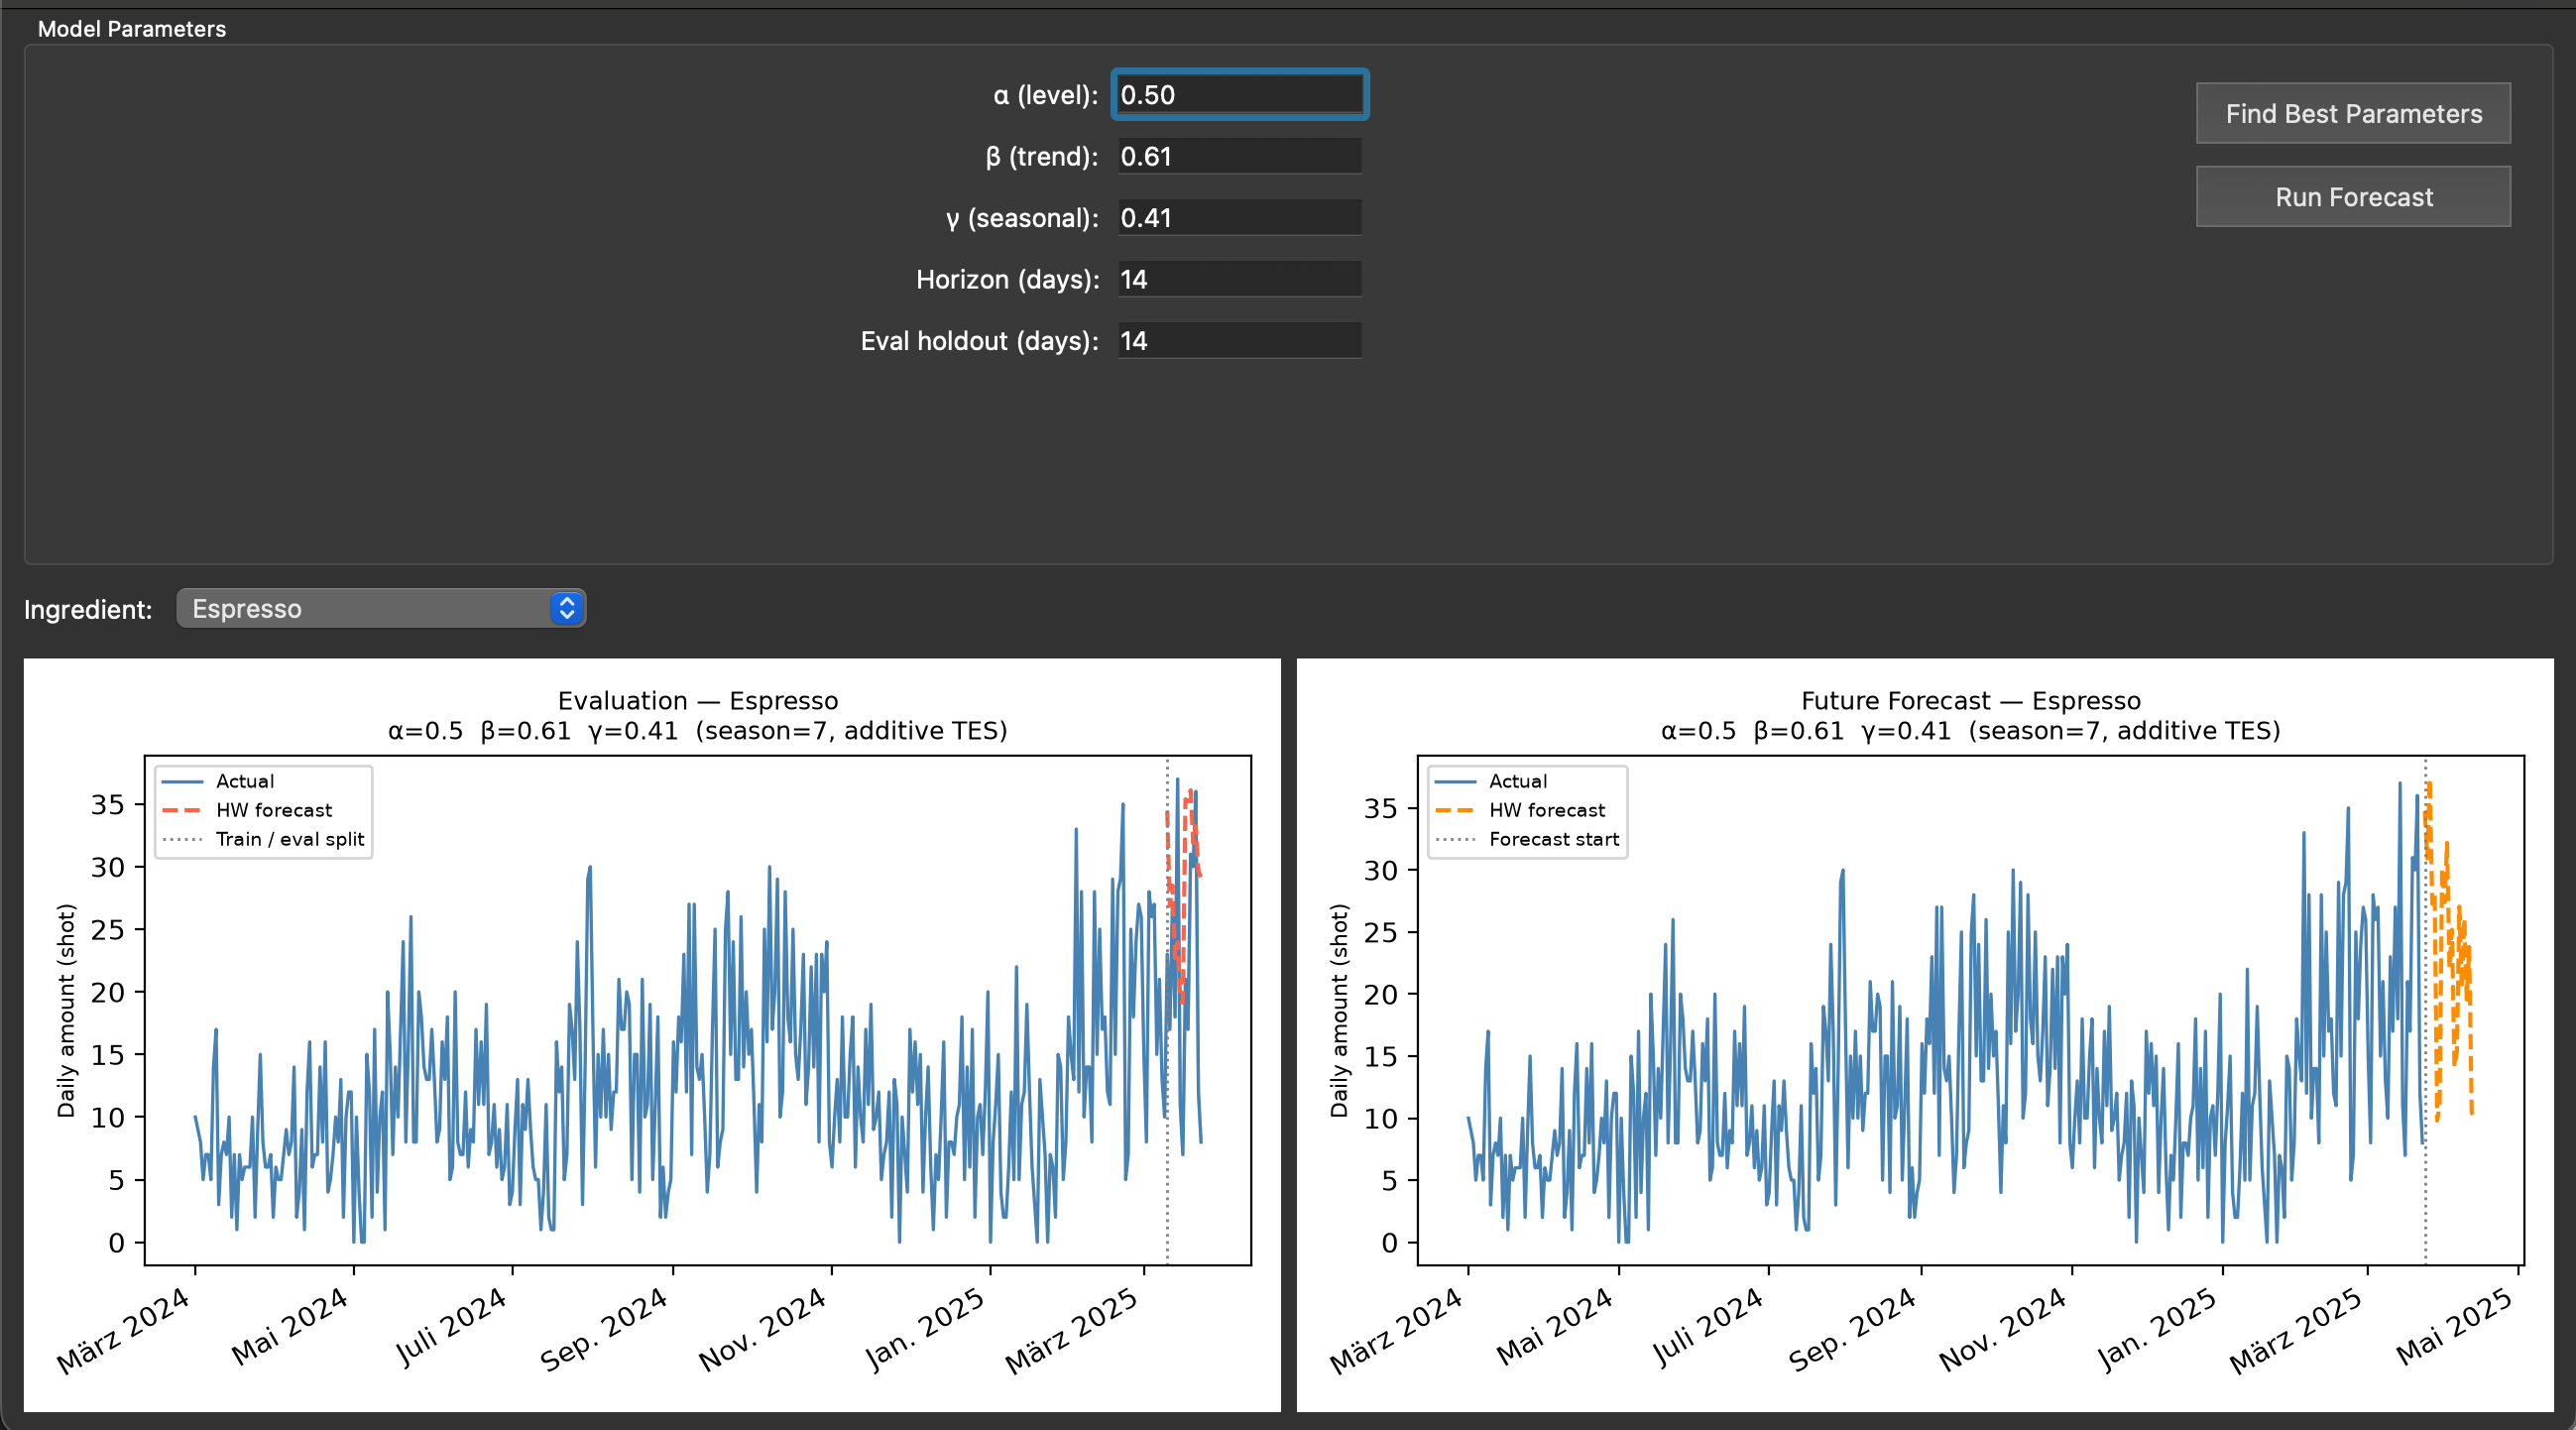
\includegraphics[width=\linewidth]{gui_screenshot.png}
    \caption{The graphical interface showing model parameters, the ingredient, and the resulting evaluation and future forecast plots.}
    \label{fig:gui}
\end{figure}
Users can interact with the demo through a graphical interface (see Fig.~\ref{fig:gui}). 
First, the user can select the parameter manually or run a grid search to find the best parameters for the forecasting model.
Afterwards, the user can run the forecasting model and visualize the results for one ingredient. For the selected ingredient 2 plots are created, one comparing actual sales against the forecast for the held-out evaluation period, and one showing the forecast for the upcoming days beyond the available data.
After the forecast is generated and without running the forecasting model again, the user can select another ingredient in a drop down menu and visualize the results for that ingredient.
Visitors are also encouraged to compare ingredients that differ in how many drinks contribute to them. Ingredients drawn from several drinks tend to produce a stable forecast, since noise in any single drink's prediction is averaged out, whereas ingredients tied to only one or two drinks can inherit that drink's forecasting errors directly. This makes it possible to observe, within the same interface, both cases where the model performs convincingly and cases where its assumptions no longer hold.
\subsection{Conclusion}
The demo shows a complete path from raw, per-cup sales records to ingredient-level forecasts that could plausibly support purchasing decisions in a small coffee shop. Its particular value lies not in presenting a single polished result, but in letting visitors interactively expose the conditions under which a common forecasting method remains reliable and the conditions under which it does not, using the same pipeline and the same data throughout

\section*{References}
References are excluded from the page limit, i.e., the bibliography might exceed the second page and it cannot be used to fill the 1.5 pages.

\end{document}
